\documentclass[a4paper, 11pt]{article}
\usepackage{float}
\usepackage{amsmath}
\usepackage{graphicx}
\usepackage{geometry}
\usepackage{listings}
\geometry{scale=0.8}
\linespread{1.5}
\usepackage{hyperref}
\usepackage{listings}


\title{	
\normalfont \normalsize
\textsc{School of Data and Computer Science, Sun Yat-sen University} \\ [25pt] %textsc small capital letters
\rule{\textwidth}{0.5pt} \\[0.4cm] % Thin top horizontal rule
\huge  E09 Bayesian Network \\ % The assignment title
\rule{\textwidth}{2pt} \\[0.5cm] % Thick bottom horizontal rule
\author{Suixin Ou \and Linkai Yang}
\date{\normalsize October 26, 2020}
}

\begin{document}
\maketitle
\tableofcontents
\newpage
\section{Pomegranate Installation}
\textbf{Under Linux:}
\begin{enumerate}
\item Install \texttt{python} first (\textbf{python 2}, not python 3).
\item Run \texttt{sudo apt-get install python-pip} to install \texttt{pip}.
\item Run \texttt{sudo pip install pomegranate} to install \texttt{pomegranate}.
\end{enumerate}
\begin{figure}[h]
  \centering
  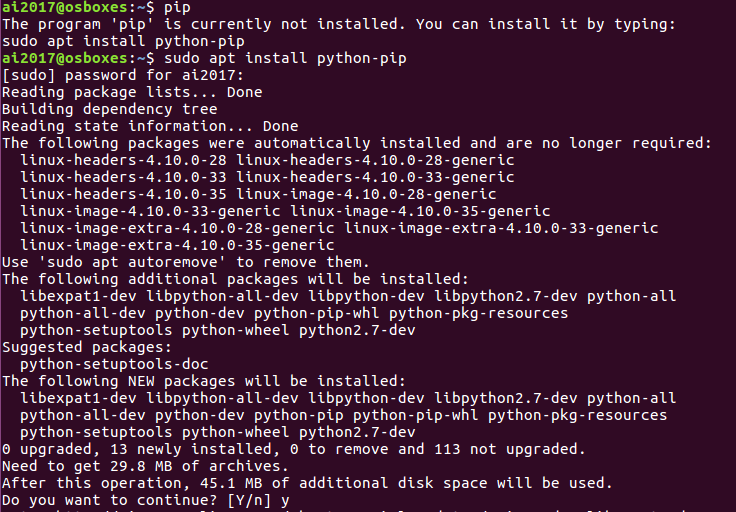
\includegraphics[width=7.5cm]{Pic/install1}
  \qquad
  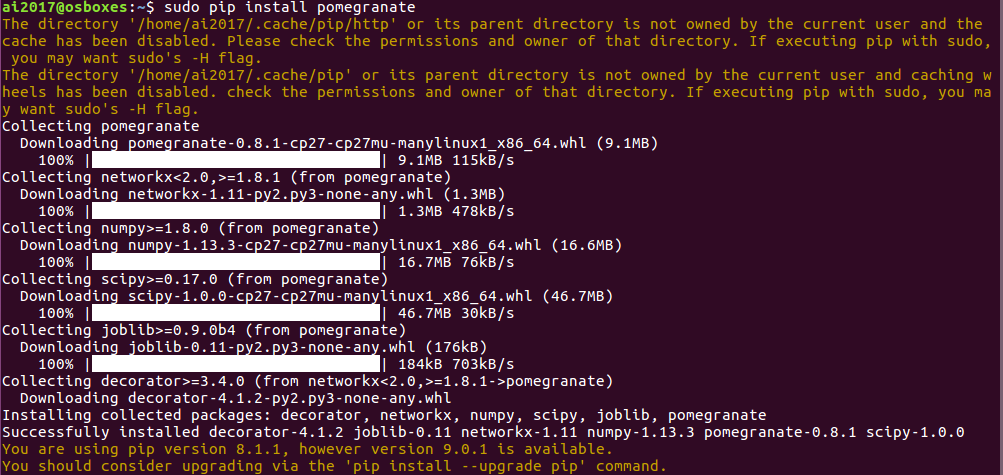
\includegraphics[width=8cm]{Pic/install2}
\end{figure}
\textbf{Under Windows}

You can also run \texttt{pip install pomegranate} if you have installed \texttt{pip}. If you don't know how to install \texttt{pip}, please click \url{https://jingyan.baidu.com/article/e73e26c0d94e0524adb6a7ff.html}.

For more, please click the homepage of Pomegranate - \url{https://github.com/jmschrei/pomegranate} for help. 
\begin{figure}[h]

  
  \centering
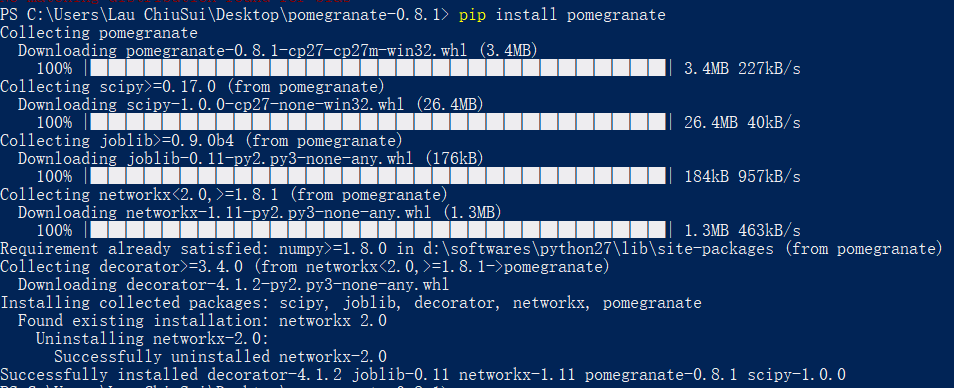
\includegraphics[width=16cm]{Pic/po}
  
\end{figure}

\section{Building Bayesian Network}
\label{sec:build-bayes-netw}
Please refer to \texttt{Tutorial\_4\_Bayesian\_Networks.pdf}. I will explain it in class.

\section{Tasks}
\label{sec:tasks}

\subsection{Burglary}
\label{sec:burglary}
\begin{figure}[h]
  \centering

  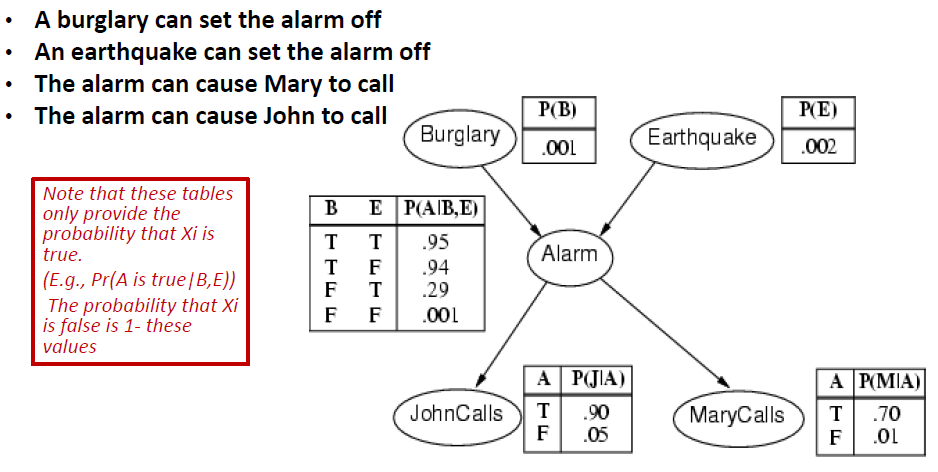
\includegraphics[width=14cm]{Pic/burglary}
\end{figure}
Please code to calculate:
\begin{enumerate}
\item $P(A)$
\item $P(J\overline{M})$
\item $P(A | J\overline{M})$
\item $P(B | A)$
  \item $P(B | J\overline{M})$
  \item  $P(J\overline{M} | \overline{B})$
\end{enumerate}
\begin{figure}[ht]
\centering
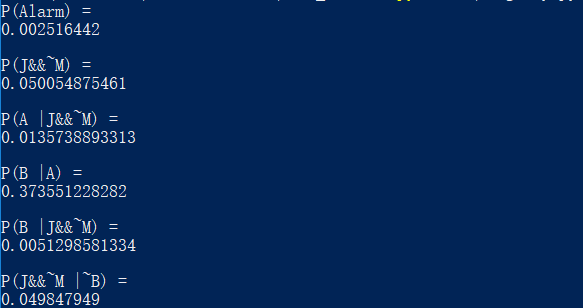
\includegraphics[width=12cm]{Pic/burglar_result}
\end{figure}
\subsection{Diagnosing}
\label{sec:bayesian-networks}
\textbf{Variables and their domais}
\begin{lstlisting}{language=Python}
(1)PatientAge:['0-30','31-65','65+']
(2)CTScanResult:['Ischemic Stroke','Hemmorraghic Stroke']
(3)MRIScanResult: ['Ischemic Stroke','Hemmorraghic Stroke']
(4)StrokeType: ['Ischemic Stroke','Hemmorraghic Stroke', 'Stroke Mimic']
(5)Anticoagulants: ['Used','Not used']
(6)Mortality:['True', 'False']
(7)Disability: ['Negligible', 'Moderate', 'Severe']
\end{lstlisting}
\textbf{CPTs}

\textbf{Note:} [CTScanResult, MRIScanResult,StrokeType] means:

P(StrokeType='...' $|$ CTScanResult='...' $\land$  MRIScanResult='...') 
\begin{lstlisting}{language=Python}
(1)
[PatientAge]

['0-30',0.10],
['31-65',0.30],
['65+',0.60]

(2)
[CTScanResult]

['Ischemic Stroke',0.7],
['Hemmorraghic Stroke',0.3]

(3)
[MRIScanResult]

['Ischemic Stroke',0.7],
['Hemmorraghic Stroke',0.3]

(4)
[Anticoagulants]

['Used',0.5],
['Not used',0.5]

(5)
[CTScanResult,MRIScanResult,StrokeType]

['Ischemic Stroke','Ischemic Stroke','Ischemic Stroke',0.8],
['Ischemic Stroke','Hemmorraghic Stroke','Ischemic Stroke',0.5],  
['Hemmorraghic Stroke','Ischemic Stroke','Ischemic Stroke',0.5],
['Hemmorraghic Stroke','Hemmorraghic Stroke','Ischemic Stroke',0], 

['Ischemic Stroke','Ischemic Stroke','Hemmorraghic Stroke',0],
['Ischemic Stroke','Hemmorraghic Stroke','Hemmorraghic Stroke',0.4], 
['Hemmorraghic Stroke','Ischemic Stroke','Hemmorraghic Stroke',0.4],
['Hemmorraghic Stroke','Hemmorraghic Stroke','Hemmorraghic Stroke',0.9],

['Ischemic Stroke','Ischemic Stroke','Stroke Mimic',0.2],
['Ischemic Stroke','Hemmorraghic Stroke','Stroke Mimic',0.1],    
['Hemmorraghic Stroke','Ischemic Stroke','Stroke Mimic',0.1],
['Hemmorraghic Stroke','Hemmorraghic Stroke','Stroke Mimic',0.1],

(6) 
[StrokeType, Anticoagulants, Mortality]

['Ischemic Stroke', 'Used', 'False',0.28],
['Hemmorraghic Stroke', 'Used', 'False',0.99],
['Stroke Mimic', 'Used', 'False',0.1],
['Ischemic Stroke','Not used', 'False',0.56],
['Hemmorraghic Stroke', 'Not used', 'False',0.58],
['Stroke Mimic', 'Not used', 'False',0.05],

['Ischemic Stroke',  'Used' ,'True',0.72],
['Hemmorraghic Stroke', 'Used', 'True',0.01],
['Stroke Mimic', 'Used', 'True',0.9],
['Ischemic Stroke',  'Not used' ,'True',0.44],
['Hemmorraghic Stroke', 'Not used', 'True',0.42 ],
['Stroke Mimic', 'Not used', 'True',0.95]

(7)
[StrokeType, PatientAge, Disability]

['Ischemic Stroke',   '0-30','Negligible', 0.80],
['Hemmorraghic Stroke', '0-30','Negligible', 0.70],
['Stroke Mimic',        '0-30', 'Negligible',0.9],
['Ischemic Stroke',     '31-65','Negligible', 0.60],
['Hemmorraghic Stroke', '31-65','Negligible', 0.50],
['Stroke Mimic',        '31-65', 'Negligible',0.4],
['Ischemic Stroke',     '65+'  , 'Negligible',0.30],
['Hemmorraghic Stroke', '65+'  , 'Negligible',0.20],
['Stroke Mimic',        '65+'  , 'Negligible',0.1],

['Ischemic Stroke',     '0-30' ,'Moderate',0.1],
['Hemmorraghic Stroke', '0-30' ,'Moderate',0.2],
['Stroke Mimic',        '0-30' ,'Moderate',0.05],
['Ischemic Stroke',     '31-65','Moderate',0.3],
['Hemmorraghic Stroke', '31-65','Moderate',0.4],
['Stroke Mimic',        '31-65','Moderate',0.3],
['Ischemic Stroke',     '65+'  ,'Moderate',0.4],
['Hemmorraghic Stroke', '65+'  ,'Moderate',0.2],
['Stroke Mimic',        '65+'  ,'Moderate',0.1],

['Ischemic Stroke',     '0-30' ,'Severe',0.1],
['Hemmorraghic Stroke', '0-30' ,'Severe',0.1],
['Stroke Mimic',        '0-30' ,'Severe',0.05],
['Ischemic Stroke',     '31-65','Severe',0.1],
['Hemmorraghic Stroke', '31-65','Severe',0.1],
['Stroke Mimic',        '31-65','Severe',0.3],
['Ischemic Stroke',     '65+'  ,'Severe',0.3],
['Hemmorraghic Stroke', '65+'  ,'Severe',0.6],
['Stroke Mimic',        '65+'  ,'Severe',0.8]
\end{lstlisting}
\textbf{Calculation}

Please code to calculate the following probability value:

p1 = P(Mortality='True' $|$ PatientAge='31-65' $\land$ CTScanResult='Ischemic Stroke')

p2 = P(Disability='Moderate' $|$ PatientAge='65+' $\land$  MRIScanResult='Hemmorraghic Stroke')

p3 = P(StrokeType='Stroke Mimic' $|$ PatientAge='65+' $\land$ CTScanResult='Hemmorraghic Stroke' $\land$ MRIScanResult='Ischemic Stroke')

p4 = P(Anticoagulants='Not used' $|$ PatientAge='0-30')

\begin{figure}[ht]
\centering
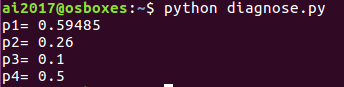
\includegraphics[width=12cm]{Pic/diagnose_result}
\end{figure}

Please solve the 2 tasks and hand in a file named \textsf{E08\_YourNumber.pdf}, and send it to \textsf{ai\_2020@foxmail.com}


\section{Codes and Results}
\subsection{Codes}
\subsubsection{Burglary}
\begin{lstlisting}[title=burglary.py,language=python,numbers=left]
from pomegranate import *
B = DiscreteDistribution({True: 0.001, False: 0.999})
E = DiscreteDistribution({True: 0.002, False: 0.998})
A = ConditionalProbabilityTable(
    [[True, True, True, 0.95],
     [True, True, False, 0.05],
     [True, False, True, 0.94],
     [True, False, False, 0.06],
     [False, True, True, 0.29],
     [False, True, False, 0.71],
     [False, False, True, 0.001],
     [False, False, False, 0.999]],
    [B, E])
J = ConditionalProbabilityTable(
    [[True, True, 0.9],
     [True, False, 0.1],
     [False, True, 0.05],
     [False, False, 0.95]],
    [A])
M = ConditionalProbabilityTable(
    [[True, True, 0.7],
     [True, False, 0.3],
     [False, True, 0.01],
     [False, False, 0.99]],
    [A])
s0 = State(B, name='B')
s1 = State(E, name='E')
s2 = State(A, name='A')
s3 = State(J, name='J')
s4 = State(M, name='M')
model = BayesianNetwork('Burglary')
model.add_states(s0, s1, s2, s3, s4)
model.add_transition(s0, s2)
model.add_transition(s1, s2)
model.add_transition(s2, s3)
model.add_transition(s2, s4)
model.bake()
PA1 = model.predict_proba({})[2].parameters[0][True]
PJ1M0 = model.predict_proba({'M': False})[
    3].parameters[0][True] * model.predict_proba({})[4].parameters[0][False]
PA1_J1M0 = model.predict_proba({'J': True, 'M': False})[2].parameters[0][True]
PB1_A1 = model.predict_proba({'A': True})[0].parameters[0][True]
PB1_J1M0 = model.predict_proba({'J': True, 'M': False})[0].parameters[0][True]
PJ1M0_B0 = (1 - PB1_J1M0) * PJ1M0 / \
    model.predict_proba({})[0].parameters[0][False]
print(PA1)
print(PJ1M0)
print(PA1_J1M0)
print(PB1_A1)
print(PB1_J1M0)
print(PJ1M0_B0)
\end{lstlisting}

\subsubsection{Diagnosing}
\begin{lstlisting}[title=diagnosing.py,language=python,numbers=left]
from pomegranate import *
PatientAge = DiscreteDistribution({'0-30': 0.10, '31-65': 0.30, '65+': 0.60})
CTScanResult = DiscreteDistribution(
    {'Ischemic Stroke': 0.7, 'Hemmorraghic Stroke': 0.3})
MRIScanResult = DiscreteDistribution(
    {'Ischemic Stroke': 0.7, 'Hemmorraghic Stroke': 0.3})
Anticoagulants = DiscreteDistribution({'Used': 0.5, 'Not used': 0.5})
StrokeType = ConditionalProbabilityTable(
    [['Ischemic Stroke', 'Ischemic Stroke', 'Ischemic Stroke', 0.8],
     ['Ischemic Stroke', 'Hemmorraghic Stroke', 'Ischemic Stroke', 0.5],
     ['Hemmorraghic Stroke', 'Ischemic Stroke', 'Ischemic Stroke', 0.5],
     ['Hemmorraghic Stroke', 'Hemmorraghic Stroke', 'Ischemic Stroke', 0],
     ['Ischemic Stroke', 'Ischemic Stroke', 'Hemmorraghic Stroke', 0],
     ['Ischemic Stroke', 'Hemmorraghic Stroke', 'Hemmorraghic Stroke', 0.4],
     ['Hemmorraghic Stroke', 'Ischemic Stroke', 'Hemmorraghic Stroke', 0.4],
     ['Hemmorraghic Stroke', 'Hemmorraghic Stroke', 'Hemmorraghic Stroke', 0.9],
     ['Ischemic Stroke', 'Ischemic Stroke', 'Stroke Mimic', 0.2],
     ['Ischemic Stroke', 'Hemmorraghic Stroke', 'Stroke Mimic', 0.1],
     ['Hemmorraghic Stroke', 'Ischemic Stroke', 'Stroke Mimic', 0.1],
     ['Hemmorraghic Stroke', 'Hemmorraghic Stroke', 'Stroke Mimic', 0.1]],
    [CTScanResult, MRIScanResult])
Mortality = ConditionalProbabilityTable(
    [['Ischemic Stroke', 'Used', 'False', 0.28],
     ['Hemmorraghic Stroke', 'Used', 'False', 0.99],
        ['Stroke Mimic', 'Used', 'False', 0.1],
        ['Ischemic Stroke', 'Not used', 'False', 0.56],
        ['Hemmorraghic Stroke', 'Not used', 'False', 0.58],
        ['Stroke Mimic', 'Not used', 'False', 0.05],
        ['Ischemic Stroke',  'Used', 'True', 0.72],
        ['Hemmorraghic Stroke', 'Used', 'True', 0.01],
        ['Stroke Mimic', 'Used', 'True', 0.9],
        ['Ischemic Stroke',  'Not used', 'True', 0.44],
        ['Hemmorraghic Stroke', 'Not used', 'True', 0.42],
        ['Stroke Mimic', 'Not used', 'True', 0.95]],
    [StrokeType, Anticoagulants])
Disability = ConditionalProbabilityTable(
    [['Ischemic Stroke',   '0-30', 'Negligible', 0.80],
     ['Hemmorraghic Stroke', '0-30', 'Negligible', 0.70],
        ['Stroke Mimic',        '0-30', 'Negligible', 0.9],
        ['Ischemic Stroke',     '31-65', 'Negligible', 0.60],
        ['Hemmorraghic Stroke', '31-65', 'Negligible', 0.50],
        ['Stroke Mimic',        '31-65', 'Negligible', 0.4],
        ['Ischemic Stroke',     '65+', 'Negligible', 0.30],
        ['Hemmorraghic Stroke', '65+', 'Negligible', 0.20],
        ['Stroke Mimic',        '65+', 'Negligible', 0.1],
        ['Ischemic Stroke',     '0-30', 'Moderate', 0.1],
        ['Hemmorraghic Stroke', '0-30', 'Moderate', 0.2],
        ['Stroke Mimic',        '0-30', 'Moderate', 0.05],
        ['Ischemic Stroke',     '31-65', 'Moderate', 0.3],
        ['Hemmorraghic Stroke', '31-65', 'Moderate', 0.4],
        ['Stroke Mimic',        '31-65', 'Moderate', 0.3],
        ['Ischemic Stroke',     '65+', 'Moderate', 0.4],
        ['Hemmorraghic Stroke', '65+', 'Moderate', 0.2],
        ['Stroke Mimic',        '65+', 'Moderate', 0.1],
        ['Ischemic Stroke',     '0-30', 'Severe', 0.1],
        ['Hemmorraghic Stroke', '0-30', 'Severe', 0.1],
        ['Stroke Mimic',        '0-30', 'Severe', 0.05],
        ['Ischemic Stroke',     '31-65', 'Severe', 0.1],
        ['Hemmorraghic Stroke', '31-65', 'Severe', 0.1],
        ['Stroke Mimic',        '31-65', 'Severe', 0.3],
        ['Ischemic Stroke',     '65+', 'Severe', 0.3],
        ['Hemmorraghic Stroke', '65+', 'Severe', 0.6],
        ['Stroke Mimic',        '65+', 'Severe', 0.8]],
    [StrokeType, PatientAge])
s0 = State(PatientAge, name='PatientAge')
s1 = State(CTScanResult, name='CTScanResult')
s2 = State(MRIScanResult, name='MRIScanResult')
s3 = State(Anticoagulants, name='Anticoagulants')
s4 = State(StrokeType, name='StrokeType')
s5 = State(Mortality, name='Mortality')
s6 = State(Disability, name='Disability')
model = BayesianNetwork('Diagnosing')
model.add_states(s0, s1, s2, s3, s4, s5, s6)
model.add_transition(s1, s4)
model.add_transition(s2, s4)
model.add_transition(s4, s5)
model.add_transition(s3, s5)
model.add_transition(s4, s6)
model.add_transition(s0, s6)
model.bake()
p1 = model.predict_proba(
    {'PatientAge': '31-65', 'CTScanResult': 'Ischemic Stroke'})\
        [5].parameters[0]['True']
p2 = model.predict_proba(
    {'PatientAge': '65+', 'MRIScanResult': 'Hemmorraghic Stroke'})\
        [6].parameters[0]['Moderate']
p3 = model.predict_proba(
    {'PatientAge': '65+', 'CTScanResult': 'Hemmorraghic Stroke',
                          'MRIScanResult': 'Ischemic Stroke'})\
                              [4].parameters[0]['Stroke Mimic']
p4 = model.predict_proba({'PatientAge': '0-30'})\
    [3].parameters[0]['Not used']
print(p1)
print(p2)
print(p3)
print(p4)
\end{lstlisting}

\subsection{Results}
\subsubsection{Burglary}
\begin{figure}[H]
  \centering
  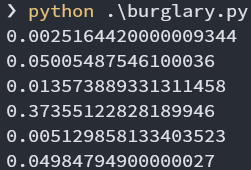
\includegraphics[width=6cm]{burglary.png}
  \caption{Result of burglary.py}
\end{figure}
\subsubsection{Diagnosing}
\begin{figure}[H]
  \centering
  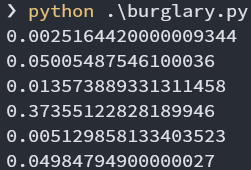
\includegraphics[width=6cm]{burglary.png}
  \caption{Result of diagnosing.py}
\end{figure}

%\clearpage
%\bibliography{E:/Papers/LiuLab}
%\bibliographystyle{apalike}
\end{document} 
%%% Local Variables:
%%% mode: latex
%%% TeX-master: t
%%% End:
